\section{Ansible}
Ansible là một giải pháp đơn giản được sử dụng trong việc tự động hóa hàng loạt các công việc liên quan đến hạ tầng CNTT như tự động cấu hình, tự động triển khai phần mềm, và nhiều công việc khác nữa. Trong mô hình của Ansible, hạ tầng CNTT của bạn được nhìn góc độ là một kiến trúc tổng thể của các thành phần có liên quan thay vì chỉ quản lý một hệ thống tại một điểm riêng lẻ. Nó không sử dụng các agent hoặc thêm vào các lớp tùy chọn bảo mật bổ sung, do đó việc triển khai Ansible vô cùng đơn giản. Một điều quan trọng nữa đó là ngôn ngữ cấu hình mà nó sử dụng rất đơn giản (được gọi là playbooks), nó cho phép mô tả những công việc tự động bằng tiếng Anh đơn thuần thay vì viết một điều gì đó phức tạp bằng một ngôn ngữ lập trình nào đó. Bằng cách sử dụng Ansible, chúng ta sẽ thực hiện việc tự động hóa hàng loạt nhanh hơn, thậm chí nó có thể đạt tới những điều mà ta chưa từng thấy trước đó.


\subsection{Tổng quan}

Ansible là một phần mềm mã nguồn mở dùng trong việc quản lý cấu hình của hạ tầng CNTT, triển khai sản phẩm công nghệ, cùng như điều phối các hoạt động tự động hóa khác. Với chỉ một công cụ duy nhất, nó đem lại những hiệu quả lớn trước hàng loạt các thách thức về tự động hóa. Ansible cung cấp sự thay thế hiệu các chức năng cốt lỗi vốn có trong các giải pháp tự động hóa khác, đồng thời tìm kiếm lời giải cho những vấn đề chưa được giải quyết. Bao gồm sự phối hợp rõ ràng về các quy trình làm việc phức tạp và sự thống nhất về cấu hình của hệ điều hành và phần mềm ứng dụng triển khai.

Ansible tìm cách giữ cho những mô tả về các quy trình công việc dễ hiểu và có thể được thực hiện nhanh chóng. Điều đó đồng nghĩa với việc những người mới sử dụng Ansbile có thể nhanh chóng hòa nhập vào các dự án mới, đồng thời dễ dàng hiểu được những công việc cho dù họ có tham gia vào dự án muộn hơn. Không chỉ vậy, Ansible luôn tìm cách tạo ra những công cụ thật mạnh mẽ cho những chuyên gia, nhưng bình đẳng cho tất cả các cấp độ kỹ năng của người sử dụng. Từ đó, rút ngắn thời gian đưa sản phẩm ra thị trường; giảm thiểu các lỗi có thể xảy ra do sự thay đổi cấu hình của hạ tầng CNTT.

Ansible được thiết kế nhỏ gọn, tiện dụng, an toàn, và có độ tin cậy cao, không mất nhiều công sức trong việc học sử dụng cho dù là quản trị viên, nhà phát triển hay nhà quản lý.

\subsection{Kiến trúc hệ thống}

\begin{figure}[h!]
    \begin{center}
    \fbox{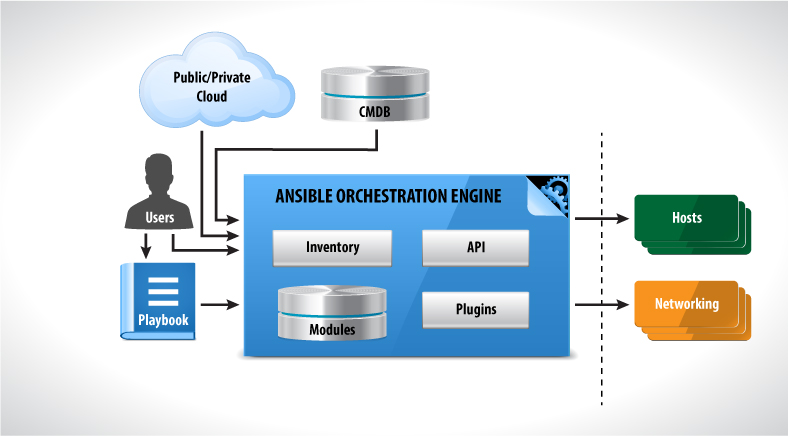
\includegraphics[width=\textwidth]{images/ansible_architect.jpg}}
    \end{center}
    \caption{Kiến trúc hệ thống của Ansible}
    \label{fig:ansible_arch}
\end{figure}

\newpage
\clearpage

Một trong những khác biệt chính giữa Ansible với những sản phẩm cùng loại chính là kiến trúc của nó

\begin{itemize}
\item Mặc định, Ansible quản lý các máy trạm thông qua giao thức SSH. Nó sử dụng một thư viện được gọi là \textbf{paramiko} (được viết bằng lập trình Python\footnote{\url{https://en.wikipedia.org/wiki/Python_(programming_language)}}) hoặc sử dụng ngay OpenSSH của hệ điều hành.

\item Ansible có thể truyền tải theo khác nhau, các phương thức là có thể thay đổi được. Ví dụ: Mặc dù \textbf{0mq} - một phương thức truyền tải tăng tốc (accelerated transport) được đưa ra nhưng Ansible hỗ trợ cả phương thức không sử dụng mạng.

\item Ansible không yêu cầu quyền root\footnote{account có quyền tuyệt đối với hệ thống trên Linux, BSD hay Solaris} để truy cập mà nó có thể cấu hình để dùng sudo\footnote{\url{https://en.wikipedia.org/wiki/Sudo}} trong các trường hợp cần thiết.

\item Ansible không yêu cầu một khóa SSH cụ thể hay một người dùng riêng. Nó có thể làm việc với bất cứ người sử dụng được cung cấp, nghĩa là Ansible tôn trọng quyền truy cập của hệ điều hành của bạn.

\item Khi có yêu cầu, Ansible sẽ chuyển các module cần thiết tới các nút điều khiển, sau đó chạy chúng từ xa với các thông tin người dùng đã được cung cấp và không để lại được bất cứ cài đặt gì trên các nút này.

\item Ansible không yêu cầu bất kỳ phần mềm máy chủ được chạy từ một máy quản lý, nó chỉ yêu cầu các thông tin đăng nhập của người dùng mà thôi.

\item Ansible không yêu cầu bất kì một phần mềm agent nào được chạy trên cái nút điều khiển.

\item Ansible không cần mở thêm bất cứ một cổng nào ngoài SSH cũng như không yêu cầu phải có hạ tầng PKI để bảo trì.

\item Những người có quyền truy cập vào máy chủ điều khiển (hoặc máy chủ điều khiển mã nguồn) không thể xóa hay thay đổi các nội dung các máy trạm (hoặc ra lệnh cho chúng chạy một lệnh nào đó) mà không có cũng có thông tin về hệ thống đó.

\item Khi không còn quản lý nữa, Ansible không dùng đến bất cứ tài nguyên nào của những máy trạm.

\end{itemize}

Những đặc điểm trên kết hợp với nhau làm cho Ansible trở nên lý tưởng cho các môi trường bảo mật hoặc hiệu suất cao, nơi có những lo ngại về sự ổn định hoặc việc thay đổi thường xuyên của các agent. Những thuộc tính trên hầu hết đều hữu ích trong các lĩnh vực về máy tính.

Ansible là sự thiết kế đồng nhất giữa kinh nghiệm của sử dụng và phương pháp tiếp cận. Ansible được thiết kế để làm cho việc cấu hình và xử lý các hạ tầng CNTT cũng chỉ đơn giản như việc đọc hoặc viết cấu hình, thậm chí đối với những người chưa qua đào tạo về việc đọc chúng.

Mặc dù Ansible có thể thực hiện hầu hết các loại nhiệm vụ tự động hóa, Ansible không giống với ngôn ngữ lập trình phần mềm, nó chỉ là các mô tả cơ bản về trạng và tiến trình. Hơn nữa, nó cố gắng để giải quyết nhiều vấn đề chồng chéo của tự động hóa hệ thống từ một framework duy nhất với mục tiêu giảm thiểu thời gian và chi phí để học và hiểu cũng như gắn kết nhiều framework với nhau.

Với các phương pháp truyền thống khác, người dùng thường phải kết hợp nhiều công cụ với nhau có để bao quát hết những điều cơ bản trong quản lý hệ thống CNTT và cấu hình phần mềm, bao gồm:

\begin{itemize}
\item Một công cụ dùng quản lý cấu hình, nó dùng để làm việc với các hệ điều hành cơ bản, mô tả các trạng thái mong muốn của một hệ thống, nhưng không phải quá trình để đưa nó vào trạng thái đó.

\item Một công cụ triển khai, dùng để đưa sản phẩm phần mềm lên hệ thống, nó tập trung vào quá trình thực hiện.

\item Một công cụ dùng để thực thi, cho các tác vụ thực thi tức thời - những thứ mà không phù hợp với mô hình trước đây, chẳng hạn như restart hàng loạt các máy chủ.
\end{itemize}

Ansible đã gộp tất cả các yếu tó đó thành một công cụ duy nhất, đồng thời cung cấp các khả năng và đặc điểm cho phép thực hiện triển khai những phần mềm nhiều lớp và các quy trình làm việc phức tạp.

\subsection{Các thành phần chính}
